\newpage

\section{Partie 1: Quelques opérations de base sur les signaux}

\subsection{Signal numérique de synthèse}

\subsubsection{Génération du signal}

Un signal sinusoïdal de fréquence \( f_0 \) est généré par la fonction suivante:

\[
x[n] = \sin\left(2\pi f_0 \frac{n}{f_e}\right)
\]

où \( f_e \) est la fréquence d’échantillonnage et \( N \) le nombre d’échantillons.

\begin{figure}[!h]
\centering
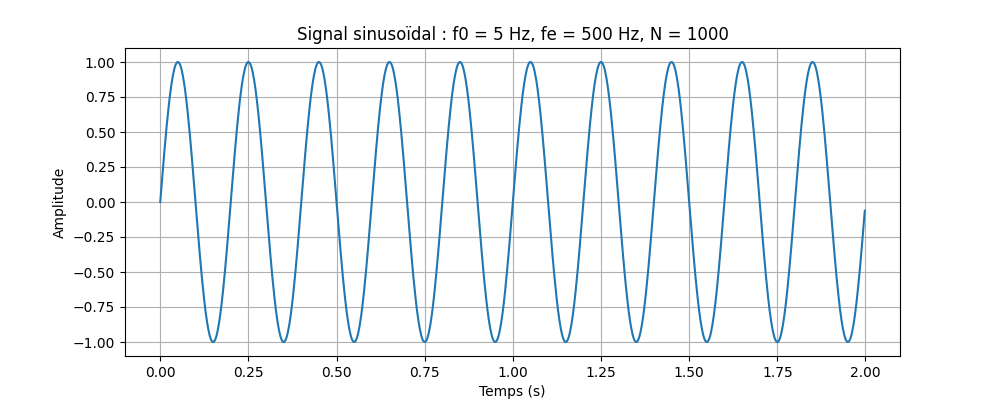
\includegraphics[width=17cm]{screenshots/signal_echantillone.png}
\caption{Signal sinusoïdal échantillonné}
\end{figure}

\subsubsection{Énergie et puissance}

L'énergie d’un signal discret \( x[n] \) est donnée par :

\[
E = \sum_{n=0}^{N-1} x[n]^2
\]

Et la puissance moyenne par :

\[
P = \frac{1}{N} \sum_{n=0}^{N-1} x[n]^2
\]

Considérons un signal sinusoïdal discret de la forme :
\[
x[n] = A \cdot \sin\left(2\pi f_0 \frac{n}{f_e} \right)
\]

La puissance moyenne théorique d’un signal périodique est calculée par la  formule:

\[
P = \lim_{N \to \infty} \frac{1}{N} \sum_{n=0}^{N-1} x[n]^2
\]

En utilisant l’identité trigonométrique :
\[
\sin^2(\theta) = \frac{1 - \cos(2\theta)}{2}
\]
on obtient :
\[
x[n]^2 = A^2 \cdot \frac{1 - \cos\left(4\pi f_0 \frac{n}{f_e} \right)}{2}
\]

Ainsi, la puissance devient :
\[
P = \lim_{N \to \infty} \frac{1}{N} \sum_{n=0}^{N-1} A^2 \cdot \frac{1 - \cos\left(4\pi f_0 \frac{n}{f_e} \right)}{2}
= \lim_{N \to \infty}  \frac{A^2}{2} - \frac{A^2}{2N} \sum_{n=0}^{N-1} \cos\left(4\pi f_0 \frac{n}{f_e} \right)
= \frac{A^2}{2}
\] 

Donc dans notre cas la puissance moyenne théorique est égale à 0.5.

Pour la puissance moyenne calculée numériquement pour le signal échantillonné on a la méme formule mais sans la limite:

\[
P = \frac{A^2}{2} - \frac{A^2}{2N} \sum_{n=0}^{N-1} \cos\left(4\pi f_0 \frac{n}{f_e} \right)
\] 

\textbf{Cas idéal :} si $N$ est un multiple entier de la période du signal (i.e., $N$ couvre un nombre entier de périodes), alors la somme des cosinus s’annule :
\[
\sum_{n=0}^{N-1} \cos\left(4\pi f_0 t \right) = 0 \quad \Rightarrow \quad P = \frac{A^2}{2}
\]

\textbf{Cas général :} si $N$ n’est pas un multiple exact de la période, la somme ne s’annule pas et on observe une légère déviation de la puissance par rapport à $\frac{A^2}{2}$. Cela est dû au fait que le signal est tronqué entre deux points non symétriques.\\

En variant N on trouve plusieurs valeurs de la puissance moyenne qui restent proches de la valeur théorique:

\begin{figure}[!h]
\centering
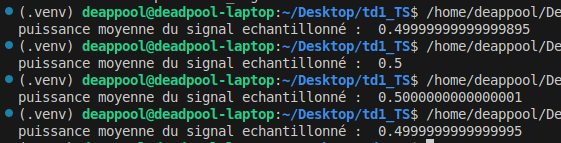
\includegraphics[width=15cm]{screenshots/puissance_et_energie.png}
\caption{Énergie et puissance du signal}
\end{figure}

\subsubsection{Quantification}

\begin{figure}[!h]
\centering
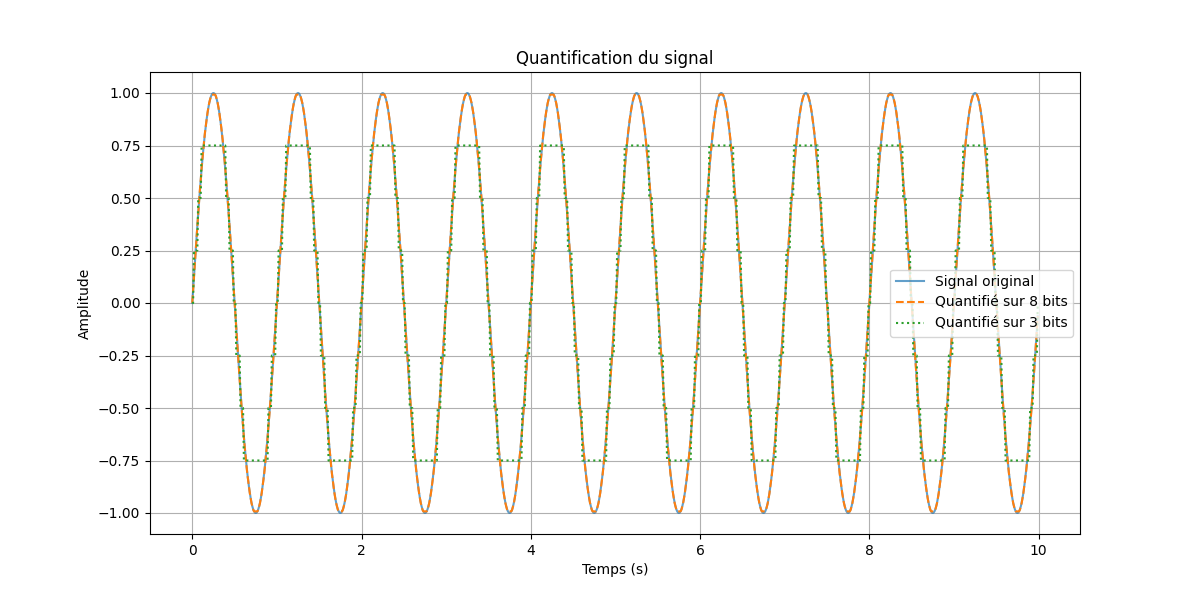
\includegraphics[width=15.5cm]{screenshots/quantification_graph.png}
\caption{Quantification du signal à 3 et 8 bits}
\end{figure}

Pour la quantification à 3 bits, on retrouve bien 8 niveaux de quantification.

\begin{figure}[!h]
\centering
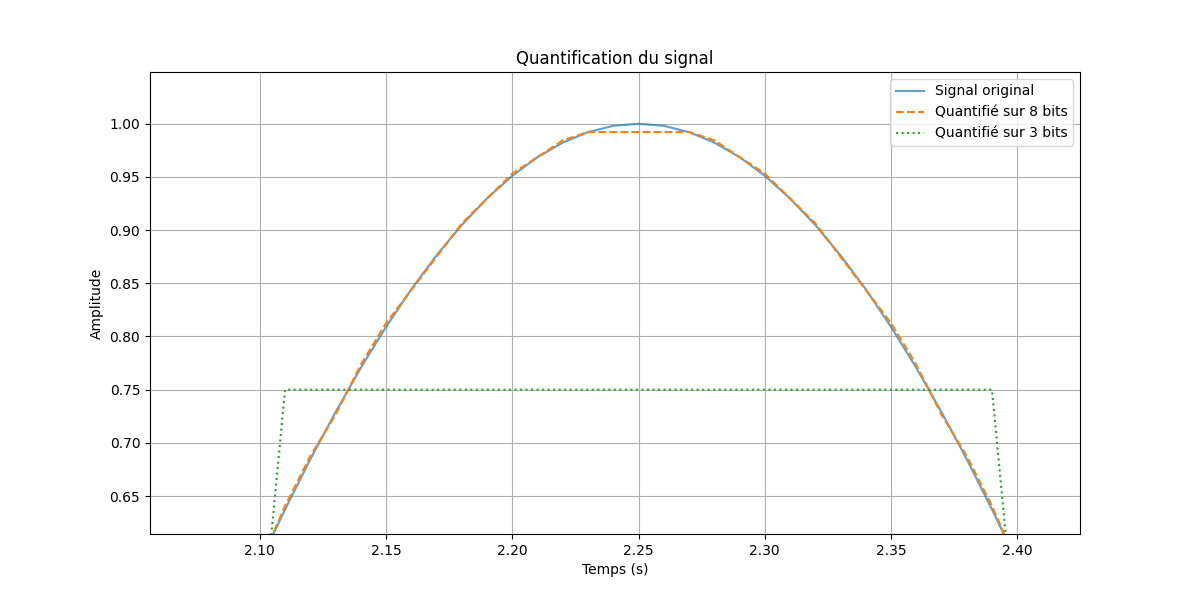
\includegraphics[width=17cm]{screenshots/quantification_graph_zoomed.png}
\caption{Zoom sur la quantification du signal à 3 et 8 bits}
\end{figure}

Le signal à 8 bits suit mieux la forme continue du signal d’origine mais on voit quand méme quelques erruers. À 3 bits, les marches sont plus visibles et le signal produit est significativement moins fidéle au signal d'origine.\\

\textbf{SNR (Signal-to-Noise Ratio)} :

\[
\text{SNR} = 10 \log_{10} \left(\frac{E_{\text{signal}}}{E_{\text{bruit}}} \right)
\]

\begin{figure}[!h]
\centering
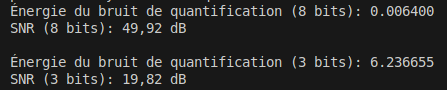
\includegraphics{screenshots/snr_quantification.png}
\caption{SNR pour chaque niveau de quantification}
\end{figure}

On remarque que l'energie du bruit est plus élevée pour le signal quantifié à 3 bits. Le résultat est logique
car on voit sur le graphe que ce signal est plus éloigné du signal d'origine comparé au signal quantifié à 8 bits.
On a la méme conclusion en raisonant sur le SNR: SNRq8 > SNRq3.

\subsection{Signal audio}

\subsubsection{Enregistrement}

Les mots « Bonjour » et « ChatGpt » ont été enregistrés via Audacity (voir figure \ref{fig:signal_enregistre}).

\subsubsection{Restitution à différentes fréquences}

L’audio est lu à \( f_e \), \( 2 f_e \) et \( \frac{f_e}{2} \). 

\textbf{Effets observés} :

\begin{itemize}
    \item \textbf{Durée :} doubler la fréquence de restitution divise la durée par deux (voix accélérée), tandis que la diviser par deux double la durée (voix ralentie).
    \item \textbf{Hauteur :} multiplier la fréquence de restitution rend la voix plus aiguë (fréquences doublées), la diminuer la rend plus grave (fréquences divisées).
\end{itemize}

Lorsque la fréquence de restitution est trop grande ou trop petite comparée à la fréquence d’échantillonnage, le son devient incompréhensible. Le son est trop rapide ou trop lent, mais aussi on ne reconnaît plus les mots. Cela s'explique notamment par le déplacement des formants, c’est-à-dire des pics de résonance caractéristiques des voyelles et consonnes, qui changent de position dans le spectre. Leur modification rend la parole méconnaissable, car ce sont eux qui permettent d’identifier les sons du langage.

\subsubsection{Quantification du signal audio}

\begin{itemize}
    \item À 3 bits : le son devient rugueux et très bruité, fortement altéré.
    \item À 8 bits : la voix reste compréhensible mais moins naturelle.
\end{itemize}

\subsubsection{Extraction et séparation de mots}

Après repérage visuel, les deux mots ont été extraits via tranches temporelles.


\begin{figure}[!h]
\centering
\includegraphics[width=10cm]{screenshots/signal_enregistré.png}
\caption{Signal audio enregistré}
\label{fig:signal_enregistre}
\end{figure}

\begin{figure}[h]
\centering
\begin{subfigure}[b]{0.45\textwidth}
    \centering
    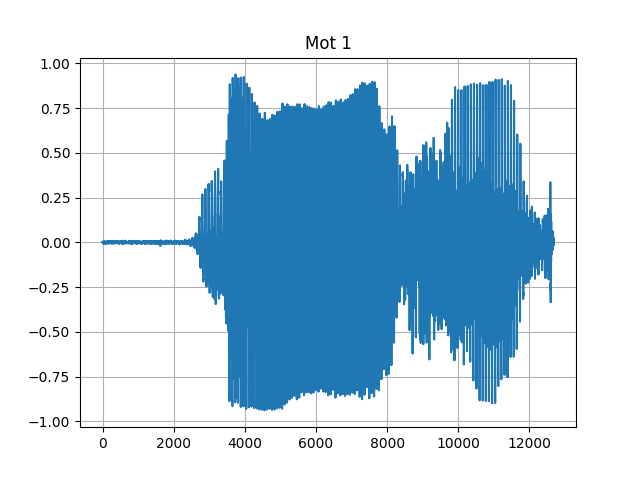
\includegraphics[width=9cm]{screenshots/mot1_graphe.png}
    \caption{Mot 1: "Bonjour"}
\end{subfigure}
\hfill
\begin{subfigure}[b]{0.45\textwidth}
    \centering
    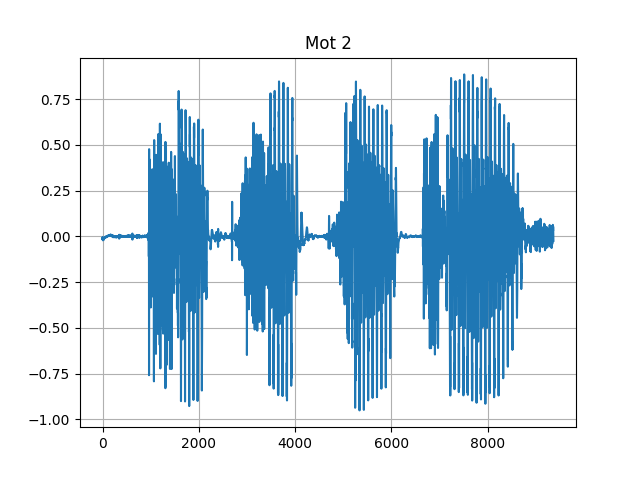
\includegraphics[width=9cm]{screenshots/mot2_graphe.png}
    \caption{Mot 2: "ChatGpt"}
\end{subfigure}
\caption{Séparation des mots dans le signal audio}
\end{figure}

\section{Partie 2: Classification des signaux}

\subsection{Exemple de calcul théorique}

Soit un signal sinusoïdal discret défini par :
\[
x[n] = A \sin(2\pi f n T_e)
\]

L'autocorrélation théorique du signal discret est définie par :
\[
R_{xx}[k] = \lim_{N \to \infty} \frac{1}{N} \sum_{n=0}^{N-1} x[n] \cdot x[n+k]
\]

En remplaçant l’expression de \( x[n] \) :
\[
R_{xx}[k] = \lim_{N \to \infty} \frac{1}{N} \sum_{n=0}^{N-1} A \sin(2\pi f n T_e) \cdot A \sin(2\pi f (n + k) T_e)
\]

\[
= A^2 \cdot \lim_{N \to \infty} \frac{1}{N} \sum_{n=0}^{N-1} \sin(2\pi f n T_e) \cdot \sin(2\pi f n T_e + 2\pi f k T_e)
\]

En utilisant l'identité trigonométrique :
\[
\sin(a)\sin(b) = \frac{1}{2} [\cos(a - b) - \cos(a + b)]
\]

On a :
\[
\sin(2\pi f n T_e) \cdot \sin(2\pi f n T_e + 2\pi f k T_e) = \frac{1}{2} \left[ \cos(2\pi f k T_e) - \cos(4\pi f n T_e + 2\pi f k T_e) \right]
\]

\[
\Rightarrow R_{xx}[k] = \frac{A^2}{2} \cos(2\pi f k T_e)
\]

car la somme de \( \cos(4\pi f n T_e + \cdot) \) sur une grande fenêtre \( N \) tend vers 0.

\textbf{Conclusion :} l'autocorrélation théorique du signal sinusoïdal discret est donnée par :
\[
\boxed{R_{xx}[k] = \frac{A^2}{2} \cos(2\pi f k T_e)}
\]

où :
\begin{itemize}
  \item \( A \) est l’amplitude du signal,
  \item \( f \) est la fréquence du signal en Hz,
  \item \( T_e = \frac{1}{f_e} \) est la période d’échantillonnage,
  \item \( k \in \mathbb{Z} \) est le décalage (lag) discret.
\end{itemize}

\subsection{Programmation}

On calcule l'autocorrélation pour un signal sinusoïdal échantillonné en utilisant la formule : 
\[
R_{xx}[k] = \frac{1}{N} \sum_{n=0}^{N-1} x[n] \cdot x[n+k]
\]

\begin{lstlisting}[language=Python]
    def autocorrelation_manual(x):
    N = len(x)
    r = np.zeros(2*N - 1)
    lags = np.arange(-N + 1, N)
    for k in range(-N + 1, N):
        somme = 0
        for n in range(N - abs(k)):
            somme += x[n] * x[n + k] if k >= 0 else x[n - k] * x[n]
        r[k + N - 1] = somme
    return lags, r
\end{lstlisting}

On compare avec l'autocorrelation calculée avec numpy et on trace la différence entre les deux résultats pour visualiser les écarts.
Pour convertir les abcisses en secondes, on utilise la formule :  
\[ \text{t} = {\text{k}}.{T_e} = \frac{\text{k}}{f_e} \]

\begin{figure}[!h]
\centering
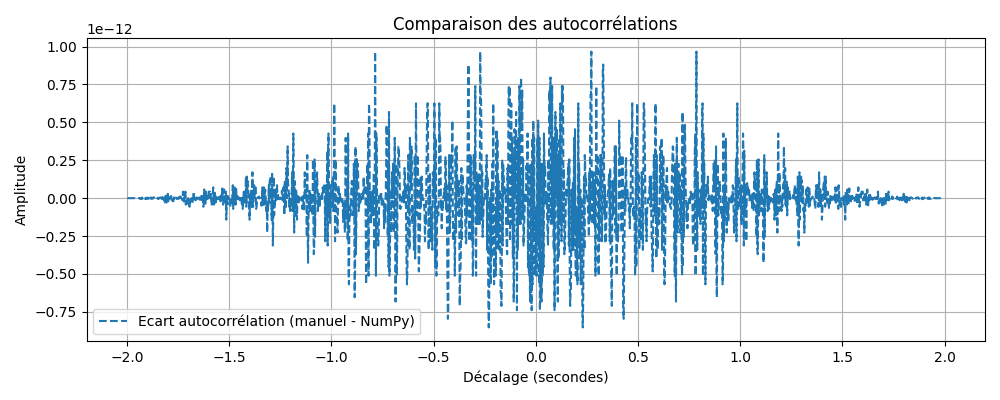
\includegraphics[width=17cm]{screenshots/ecart_autocorrelation.png}
\caption{Ecart entre l'autocorrélation manuelle et celle de numpy}
\end{figure} 

L'ecart est trop petit entre les deux méthodes (de l'ordre de \(10^{-12}\)). Ceci est dû à la précision numérique des calculs et au fait que l'autocorrelation numpy est calculée différemment en utilisant plusieurs techniques d'optimisation.\\

On calcule le rapport des énergies entre la différence entre les deux méthodes et l'autocorrelation de numpy:
\[ \text{rapport} = \frac{\sum_{k=0}^{N-1} \text{diff}[k]^2}{\sum_{k=0}^{N-1} \text{autocorr}[k]^2} \] \\

On trouve plusieurs valeurs de rapport pour différentes valeurs de N. Ceci est dû à la variation de l'énergie du signal en fonction de N, car l'autocorrelation et l'énergie sont sensibles à la longueur du signal (somme de 0 à N-1). On rajoute donc des valeurs au numérateur et au dénominateur dans le calcul de ce rapport (qui ne sont pas équivalentes vu l'écart entre les deux méthodes) ce qui expliques des valeurs de rapport différentes.

\begin{figure}[!h]
\centering
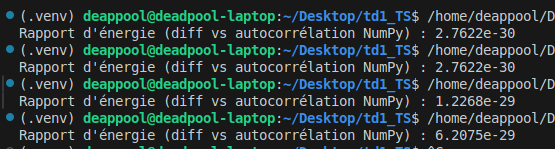
\includegraphics[width=15cm]{screenshots/valeur_rapport.png}
\caption{Valeurs du rapport pour plusieurs valeurs de N}
\end{figure} 

\subsection{Application à la classification de quelques signaux simples}

On génére les signaux demandés avec le code suivant :
\newpage
\begin{lstlisting}[language=Python]
# Parametres communs
fe = 11000          # frequence d'echantillonnage
duration = 1     # duree en secondes
t = np.linspace(0, duration, int(fe * duration), endpoint=False)

# 1. Signal sinusoidal de 200 Hz
f = 200
sinus = np.sin(2 * np.pi * f * t)

# 2. Signal triangulaire centre en 0 (serie de Fourier avec 10 termes)
tri = np.zeros_like(t)
for k in range(1, 11):
    n = 2 * k - 1  # uniquement les harmoniques impaires
    tri += ((-1)**((k+1)) / n**2) * np.sin(2 * np.pi * n * f * t)
tri *= (8 / (np.pi**2))  # normalisation serie de Fourier

# 3. Bruit blanc gaussien
taille = fe  # 1 seconde
bruit = np.random.randn(taille)
bruit /= np.max(np.abs(bruit))  # normalisation pour eviter la saturation
\end{lstlisting}

\begin{figure}[!h]
\centering
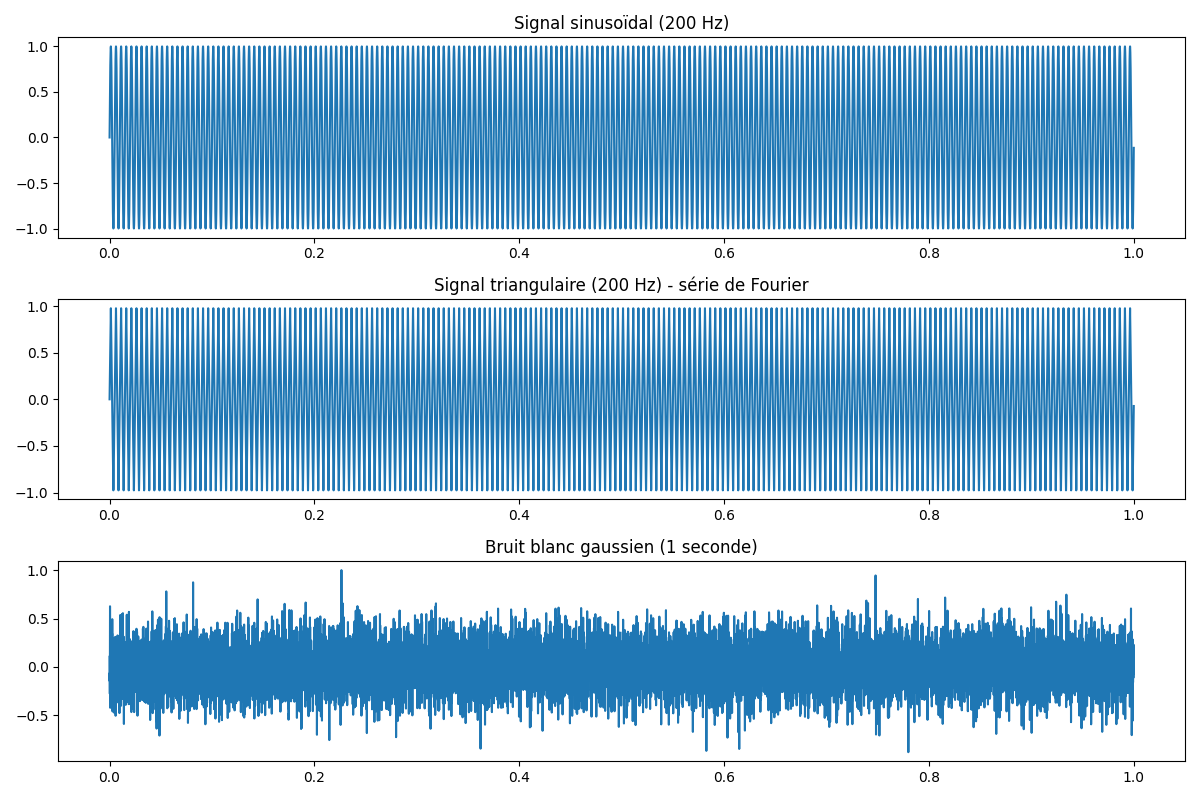
\includegraphics[width=17cm]{screenshots/generation_signaux.png}
\caption{Signaux générés}
\end{figure} 

\begin{figure}[!h]
\centering
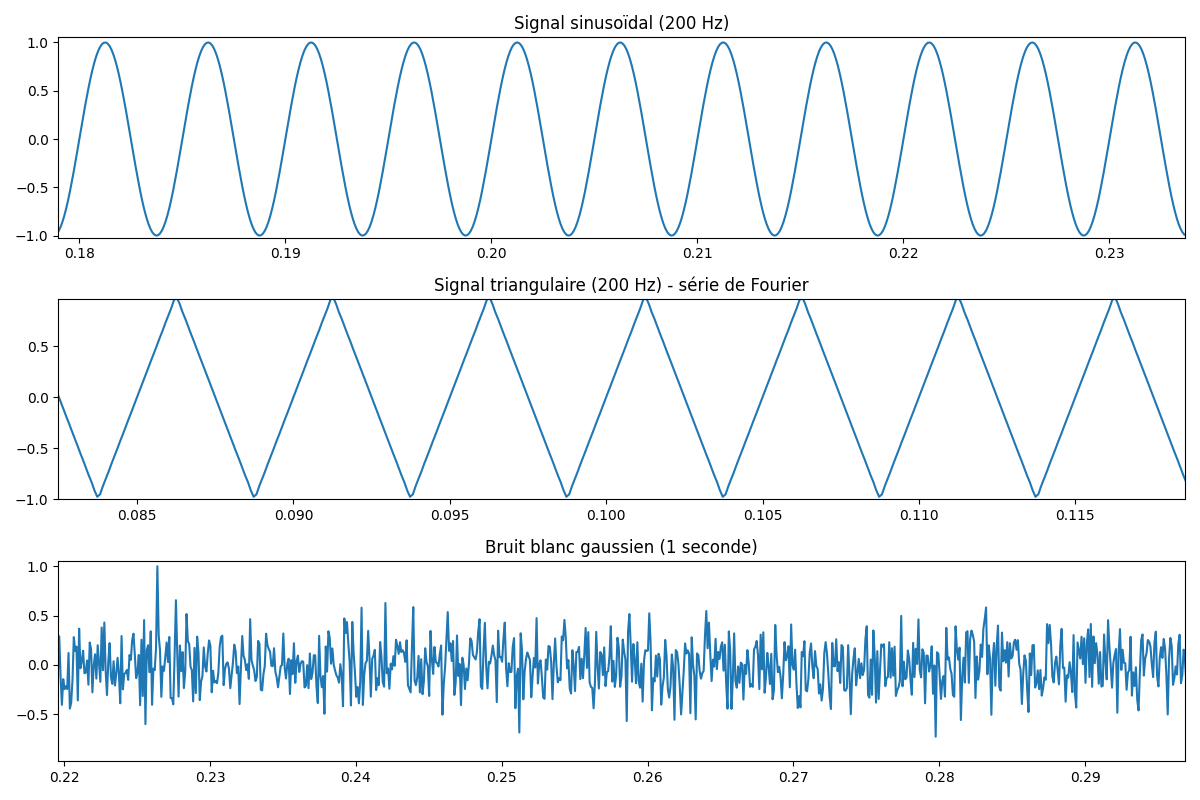
\includegraphics[width=17cm]{screenshots/generation_signaux_zoom.png}
\caption{Signaux générés (zoom)} 
\end{figure} 

\newpage

On calcule l'autocorrélation pour chaque signal sur une partie de durée de 30ms. C’est une durée typique en traitement du signal pour analyser la parole (équilibre entre résolution temporelle et fréquence). Elle est suffisante pour voir une structure (formants, périodicité...) sans mélanger des parties trop différentes du signal. On trace également l'autocorrélation du signal enregistré sur deux tranches de 30ms (et 80ms) à des moments différents (1000ms et 1500ms). Cela nous permettera de de comparer l'autocorrélation à différents moments afin de mettre en oeuvre la non-stationnarité du signal.\\

Un signal est dit \textbf{stationnaire} si ses propriétés statistiques, telles que la moyenne, la variance et l'autocorrélation, ne varient pas dans le temps.\\

L'analyse des autocorrélations montre que :
\begin{itemize}
    \item Le signal vocal « aa » est \textbf{non stationnaire} car ses caractéristiques changent entre différentes tranches temporelles (voix humaine évolue dans le temps).
    \item Le signal de bruit blanc gaussien est \textbf{stationnaire}, ses propriétés statistiques étant constantes dans le temps (Pic au centre, décroissance rapide).
    \item Les signaux sinusoïdal et triangulaire, synthétisés sur quelques périodes, sont également \textbf{stationnaires} car ils sont périodiques et leurs statistiques ne varient pas dans le temps.
\end{itemize}

\begin{figure}[!h]
\centering
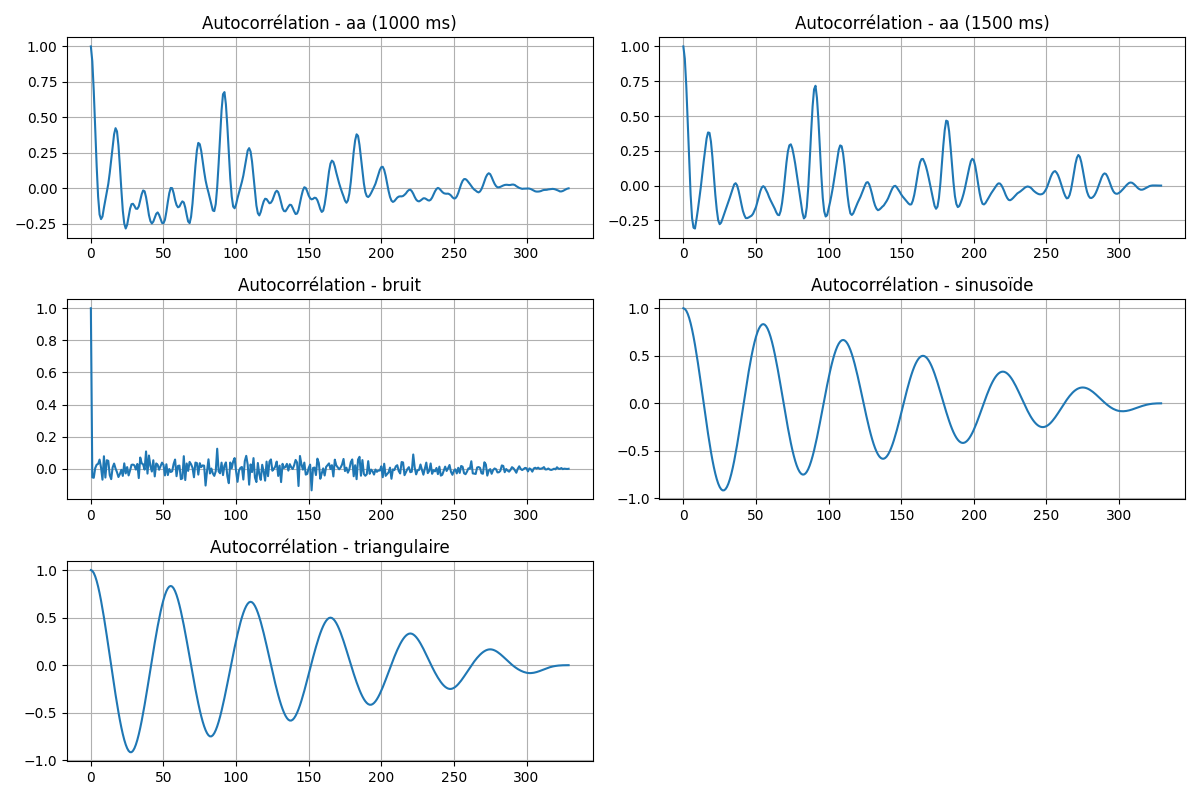
\includegraphics[width=17cm]{screenshots/autocorr_signaux_30ms.png}
\caption{autocorrélation des signaux sur 30ms} 
\end{figure} 

\begin{figure}[!h]
\centering
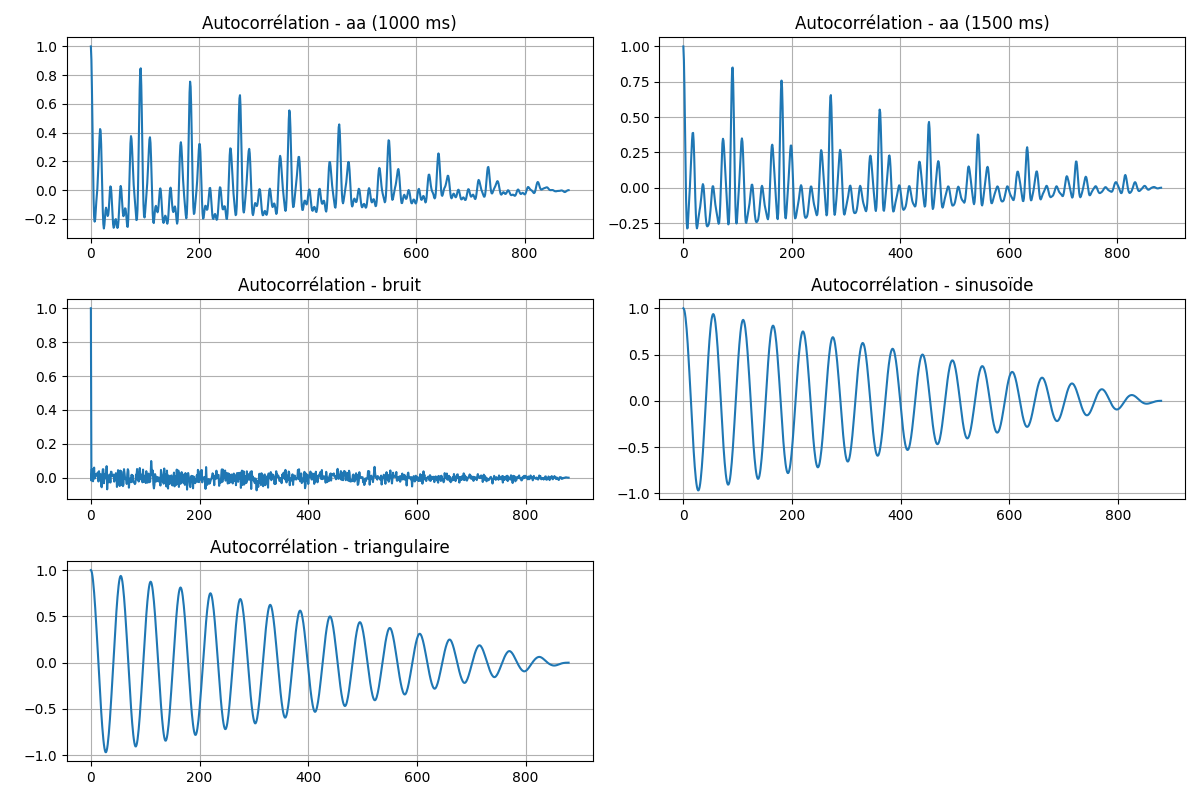
\includegraphics[width=17cm]{screenshots/autocorr_signaux_80ms.png}
\caption{autocorrélation des signaux sur 80ms} 
\end{figure}

\newpage
\subsection{Classification de signaux de parole voisés ou non voisés}

Le signal est découpé en tranches de 30 ms pour analyser leur autocorrélation. Les résultats montrent clairement deux types de comportements :

\begin{itemize}
    \item \textbf{Parties non voisées} (« chhhhh ») : l'autocorrélation est bruitée, sans périodicité marquée, caractéristique des sons fricatifs.
    \item \textbf{Parties voisées} (« aaaa ») : l'autocorrélation présente des pics réguliers, révélant une structure périodique due à la vibration des cordes vocales.
\end{itemize}

\begin{figure}[h!]
    \centering
    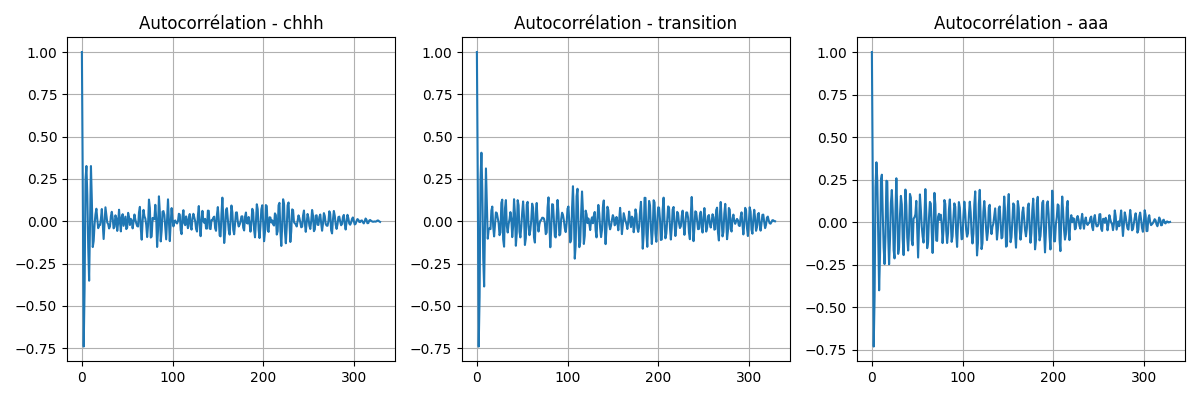
\includegraphics[width=17cm]{screenshots/autocorrelation_chat_2.png}
    \caption{Autocorrélation de différentes tranches du mot « chat » : (gauche) non voisée, (milieu) transition, (droite) voisée.}
\end{figure}


L’autocorrélation permets d'estimer la fréquence fondamentale \(f_0\) d’un signal voisé. On s’attend à ce qu’un signal périodique présente un maximum secondaire au retard correspondant à sa période fondamentale \(T_0 = \frac{1}{f_0}\).\\

Pour identifier les pics secondaires dans l’autocorrélation, nous utilisons la fonction \verb|find_peaks| de \texttt{scipy.signal}.
Afin d’éviter de détecter des pics non significatifs dus au bruit ou à des résonances (formants), deux paramètres doivent être soigneusement choisis :

\begin{itemize}
    \item \textbf{distance minimale} entre les pics, choisie pour rejeter les pics trop proches de \(t = 0\), qui ne peuvent pas correspondre à une fréquence fondamentale réaliste. On impose donc une période fondamentale minimale correspondant à une fréquence maximale plausible pour la voix humaine, généralement estimée à environ 400 Hz. Cela conduit à une période minimale d’une voix humaine raisonnable \(T_{0,\min} = \frac{1}{f_{0,\max}} = \frac{1}{400\,\mathrm{Hz}} \Rightarrow \text{distance} = \frac{f_e}{f_{0,\max}} \approx 40\) échantillons.
    \item \textbf{hauteur minimale} des pics : après normalisation de l’autocorrélation (valeur maximale = 1), on impose que seuls les pics avec une amplitude supérieure à 0{,}1 soient retenus, pour éviter de détecter du bruit.
\end{itemize}

On utilise donc: 

\begin{lstlisting}[language=python]
    peaks, _ = find_peaks(ac, height=0.05, distance=40)
\end{lstlisting}

Pour la tranche correspondant à la voyelle \textit{« a »} dans l’enregistrement (partie voisée), nous obtenons après traitement:

\begin{itemize}
    \item Indices des 4 premiers pics détectés : \([5,\ 59,\ 119,\ 199]\)
    \item Le premier pic au-delà de 40 échantillons est à \(\text{lag} = 59\)
    \item On en déduit une fréquence fondamentale :
    \[
    f_0 = \frac{f_e}{\text{lag}} = \frac{16\,000}{59} \approx 271{,}2\ \mathrm{Hz}
    \]
\end{itemize}

Sachant que l'enregistrement a été réalisé par un homme, on s’attend normalement à une fréquence fondamentale située entre 85 et 180 Hz. La valeur mesurée de 271 Hz est donc relativement élevée, ce qui peut s’expliquer par une voyelle très accentuée, un enregistrement particulier ou une éventuelle confusion dans la détection du pic de l’autocorrélation.
Mais cette valeur reste plausible pour une voix humaine adulte et correspond à une vibration régulière des cordes vocales.

\begin{figure}[h!]
    \centering
    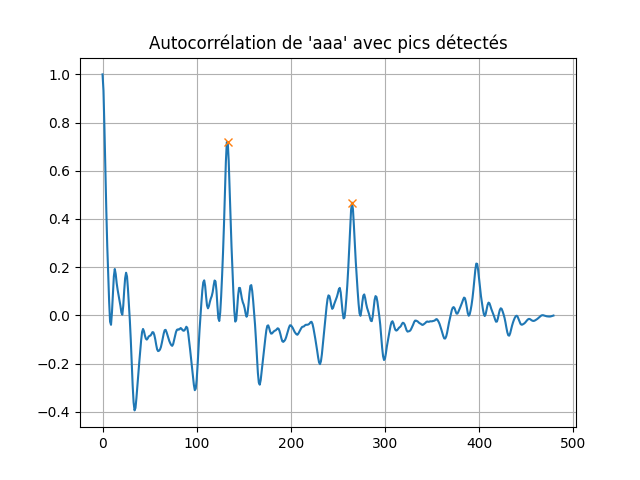
\includegraphics[width=17cm]{screenshots/autocorrelation_avec_pics_detectes.png}
    \caption{Autocorrélation de la tranche analysée avec les pics détectés.}
\end{figure}

\section{Partie 3: Aspects fréquentiels}
\subsection{Echantillonnage}

